% Tiki-Taka -- technical document, More than a Hack 2027, Phase 1 (ball possession)
% Compile: pdflatex Tiki-Taka.tex  (twice, for the references)   or   latexmk -pdf Tiki-Taka.tex
\documentclass[10pt,a4paper]{article}

% ---------------------------------------------------------------- packages
\usepackage[a4paper,margin=2.1cm,top=2.2cm,bottom=2.4cm]{geometry}
\usepackage[T1]{fontenc}
\usepackage[utf8]{inputenc}
\usepackage{lmodern}
\usepackage{microtype}
\usepackage{amsmath,amssymb}
\usepackage{booktabs,tabularx,array,multirow}
\usepackage{enumitem}
\usepackage{xcolor}
\usepackage{caption}
\usepackage{float}
\usepackage[section,above]{placeins}   % a float never leaves its section or rises above its heading
\usepackage{titlesec}
\usepackage{fancyhdr}
\usepackage{listings}
\usepackage{tikz}
\usetikzlibrary{positioning,arrows.meta,fit,backgrounds,calc,shapes.geometric,decorations.pathreplacing}
\usepackage{pgfplots}
\pgfplotsset{compat=1.18}
\usepackage[colorlinks=true,linkcolor=accent,urlcolor=accent,citecolor=accent]{hyperref}

% ---------------------------------------------------------------- look
\definecolor{accent}{HTML}{1F4E79}
\definecolor{barca}{HTML}{A50044}
\definecolor{athletic}{HTML}{D52B1E}
\definecolor{inbox}{HTML}{E8EEF5}
\definecolor{learn}{HTML}{FCE9D9}
\definecolor{learnline}{HTML}{C55A11}
\definecolor{rule}{HTML}{E2F0D9}
\definecolor{ruleline}{HTML}{548235}
\definecolor{dec}{HTML}{EDE4F3}
\definecolor{decline}{HTML}{7030A0}
\definecolor{grey}{HTML}{595959}
\definecolor{codebg}{HTML}{F5F5F5}

\titleformat{\section}{\large\bfseries\color{accent}}{\thesection}{0.6em}{}
\titleformat{\subsection}{\normalsize\bfseries\color{accent}}{\thesubsection}{0.6em}{}
\titlespacing*{\section}{0pt}{1.0em}{0.4em}
\titlespacing*{\subsection}{0pt}{0.7em}{0.25em}

% floats: let figures sit with the text and share pages instead of leaving half-empty pages
\renewcommand{\topfraction}{0.9}
\renewcommand{\bottomfraction}{0.8}
\renewcommand{\textfraction}{0.07}
\renewcommand{\floatpagefraction}{0.85}
\setcounter{topnumber}{3}
\setcounter{bottomnumber}{2}
\setcounter{totalnumber}{5}
\setlength{\textfloatsep}{10pt plus 2pt minus 3pt}
\setlength{\floatsep}{8pt plus 2pt minus 2pt}
\setlength{\intextsep}{8pt plus 2pt minus 2pt}
\setlength{\abovecaptionskip}{4pt}
\setlength{\belowcaptionskip}{0pt}
\setlist{itemsep=2pt,topsep=3pt,leftmargin=1.3em}
\captionsetup{font=small,labelfont={bf,color=accent},width=0.95\linewidth}
\setlength{\parskip}{0.25em}
\setlength{\parindent}{0pt}

\pagestyle{fancy}
\fancyhf{}
\fancyhead[L]{\small\color{grey}Tiki-Taka \textperiodcentered{} Technical document}
\fancyhead[R]{\small\color{grey}More than a Hack 2027 \textperiodcentered{} Phase 1}
\fancyfoot[C]{\small\color{grey}\thepage}
\renewcommand{\headrulewidth}{0.3pt}

\lstset{basicstyle=\ttfamily\footnotesize,backgroundcolor=\color{codebg},frame=single,
        rulecolor=\color{codebg},breaklines=true,columns=fullflexible,xleftmargin=4pt,
        xrightmargin=4pt,aboveskip=6pt,belowskip=6pt,showstringspaces=false}

\newcommand{\code}[1]{\texttt{\small #1}}
\newcommand{\sF}{spellF1}
\newcommand{\mF}{macroF1}

% TikZ styles shared by the diagrams
\tikzset{
  box/.style={draw=accent,fill=inbox,rounded corners=2pt,align=center,font=\footnotesize,
              minimum height=8mm,inner sep=3pt},
  lbox/.style={box,draw=learnline,fill=learn},
  rbox/.style={box,draw=ruleline,fill=rule},
  dbox/.style={box,draw=decline,fill=dec},
  arr/.style={-{Stealth[length=2.2mm]},thick,color=grey},
  note/.style={font=\scriptsize\itshape,color=grey,align=center},
  layer/.style={draw=learnline,fill=learn,rounded corners=1.5pt,align=center,font=\scriptsize,
                minimum width=26mm,minimum height=6.5mm,inner sep=2pt},
}

% ================================================================= document
\begin{document}

\begin{center}
  {\LARGE\bfseries\color{accent} Tiki-Taka}\\[3pt]
  {\large Frame-level ball possession from tracking data}\\[4pt]
  {\small\color{grey} More than a Hack 2027, Phase 1 \textperiodcentered{} FC Barcelona vs Athletic Club
  \textperiodcentered{} submission \code{Tiki-Taka.csv} (\code{v31\_d1\_c1dldm05\_e3k\_kt})}
\end{center}
\suppressfloats[t]   % nothing floats above the title

\vspace{2pt}
\noindent\colorbox{inbox}{\parbox{\dimexpr\linewidth-2\fboxsep}{\small
\textbf{Summary.} A hand-built evidence model and a three-state Viterbi decoder, on top of which
learned components (touch detector, team models, dead-ball head, change network, short-possession
network) are added one at a time. Every learned piece is trained on external open tracking data
(DFL, SkillCorner, PFF) and kept only if it wins on held-out external matches; the public
five-minute window is a correctness check. \textbf{Public window:} \sF{} 0.787, \mF{} 0.934.
\textbf{Held out on external data:} SkillCorner 0.6699, PFF 0.6916, DFL 0.6438. The repository
rebuilds the submitted file byte for byte (\S\ref{sec:repro}).}}

% ----------------------------------------------------------------
\section{The problem and our approach}

Every frame of the tactical video (199{,}319 frames at 25\,fps) gets \code{H}, \code{A}, \code{D}
(dead ball) or \code{X}. The ranking metric, \sF, matches whole possessions as intervals at IoU
thresholds 0.3--0.7. Two consequences shaped everything:

\begin{itemize}
  \item \textbf{Flicker is expensive.} One wrong frame barely moves \mF, but a one-second flicker
        splits a possession and can cost two matched spells. Long, clean runs matter more than
        per-frame accuracy, so the output of every model goes through a decoder that charges for
        each change of state.
  \item \textbf{There is almost no in-match supervision.} Only 17 public possessions are
        labelled. A network cannot be trained or selected on them, and the public score has
        ranked our versions wrongly before. We therefore train on external matches, prepared to
        look like ours (blurred ball, our pattern of tracking gaps, an animated dead ball), and
        select on \emph{held-out external matches}. The public window only confirms that nothing
        broke.
\end{itemize}

\textbf{Why this shape.} Proximity is not control: the organisers' nearest-player baseline
(\code{smooth50}) scores \sF{} 0.2433 because a ball between two players flickers. Who \emph{touched}
the ball last is right far more often than who is nearest (81\% vs 57\% inside short possessions
in our early tests), so team evidence is built from touches. A single end-to-end network was
not an option without in-match labels; instead each learned component is a separate expert that
feeds the same decoder, and each was validated on its own (leave-one-match-out or fixed folds).

% ----------------------------------------------------------------
\section{Pipeline}

Figure~\ref{fig:pipeline} shows the chain that produces the submitted file. The ball is not seen
on 43\% of our match's frames, which is why most stages read the players as well as the ball.

\begin{figure}[!htbp]
\centering
\resizebox{0.96\linewidth}{!}{%
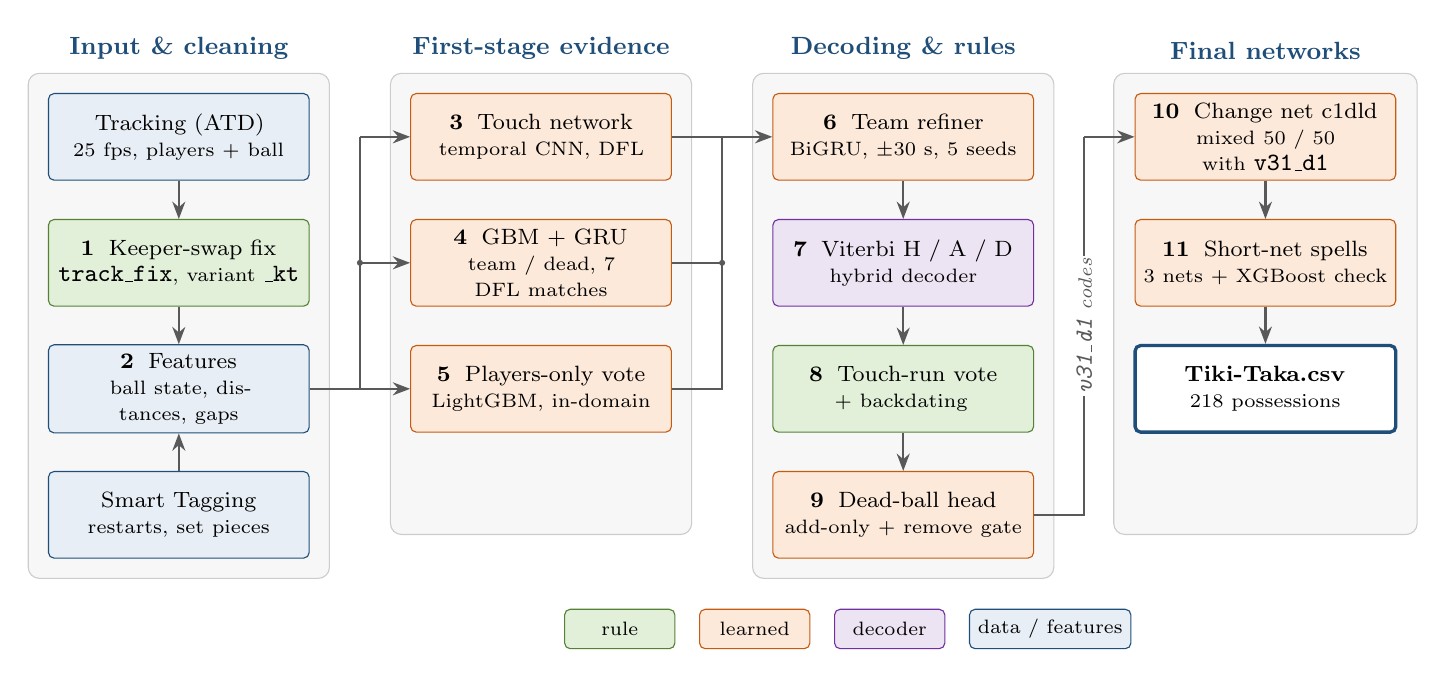
\begin{tikzpicture}[
    pn/.style={text width=31mm,minimum height=11mm},
    panel/.style={draw=gray!40,fill=gray!6,rounded corners=4pt,inner sep=2.5mm},
    ptitle/.style={font=\small\bfseries,text=accent,above,yshift=0.5mm},
    bus/.style={thick,color=grey}]
  % grid: columns at x = 0 / 4.6 / 9.2 / 13.8 cm, rows at y = 0 / -1.6 / -3.2 / -4.8 cm
  % column 1: input and cleaning
  \node[box,pn]  (atd)  at (0,0)     {Tracking (ATD)\\ \scriptsize 25 fps, players + ball};
  \node[rbox,pn] (kt)   at (0,-1.6)  {\textbf{1}\; Keeper-swap fix\\ \scriptsize \code{track\_fix}, variant \code{\_kt}};
  \node[box,pn]  (feat) at (0,-3.2)  {\textbf{2}\; Features\\ \scriptsize ball state, distances, gaps};
  \node[box,pn]  (tag)  at (0,-4.8)  {Smart Tagging\\ \scriptsize restarts, set pieces};
  % column 2: first-stage evidence
  \node[lbox,pn] (touch) at (4.6,0)    {\textbf{3}\; Touch network\\ \scriptsize temporal CNN, DFL};
  \node[lbox,pn] (gbm)   at (4.6,-1.6) {\textbf{4}\; GBM + GRU\\ \scriptsize team / dead, 7 DFL matches};
  \node[lbox,pn] (po)    at (4.6,-3.2) {\textbf{5}\; Players-only vote\\ \scriptsize LightGBM, in-domain};
  % column 3: decoding and rules
  \node[lbox,pn] (ref)   at (9.2,0)    {\textbf{6}\; Team refiner\\ \scriptsize BiGRU, $\pm$30 s, 5 seeds};
  \node[dbox,pn] (vit)   at (9.2,-1.6) {\textbf{7}\; Viterbi H / A / D\\ \scriptsize hybrid decoder};
  \node[rbox,pn] (rules) at (9.2,-3.2) {\textbf{8}\; Touch-run vote\\ \scriptsize + backdating};
  \node[lbox,pn] (dead)  at (9.2,-4.8) {\textbf{9}\; Dead-ball head\\ \scriptsize add-only + remove gate};
  % column 4: final networks
  \node[lbox,pn] (cn)  at (13.8,0)    {\textbf{10}\; Change net c1dld\\ \scriptsize mixed 50 / 50 with \code{v31\_d1}};
  \node[lbox,pn] (sn)  at (13.8,-1.6) {\textbf{11}\; Short-net spells\\ \scriptsize 3 nets + XGBoost check};
  \node[box,pn,draw=accent,very thick,fill=white] (out) at (13.8,-3.2) {\textbf{Tiki-Taka.csv}\\ \scriptsize 218 possessions};

  % panels (all the same height: they span to the bottom row)
  \coordinate (b1) at (0,-4.8);  \coordinate (b2) at (4.6,-4.8);
  \coordinate (b3) at (9.2,-4.8); \coordinate (b4) at (13.8,-4.8);
  \begin{scope}[on background layer]
    \node[panel,fit=(atd)(tag)]       (P1) {}; \node[ptitle] at (P1.north) {Input \& cleaning};
    \node[panel,fit=(touch)(po)(b2)]  (P2) {}; \node[ptitle] at (P2.north) {First-stage evidence};
    \node[panel,fit=(ref)(dead)]      (P3) {}; \node[ptitle] at (P3.north) {Decoding \& rules};
    \node[panel,fit=(cn)(out)(b4)]    (P4) {}; \node[ptitle] at (P4.north) {Final networks};
  \end{scope}

  % column 1, top to bottom; tagging feeds the features from below
  \draw[arr] (atd) -- (kt);
  \draw[arr] (kt) -- (feat);
  \draw[arr] (tag) -- (feat);
  % features -> every first-stage model (bus at x = 2.3)
  \draw[bus] (feat.east) -- (2.3,-3.2);
  \draw[bus] (2.3,-3.2) -- (2.3,0);
  \draw[arr] (2.3,0) -- (touch.west);
  \draw[arr] (2.3,-1.6) -- (gbm.west);
  \draw[arr] (2.3,-3.2) -- (po.west);
  \fill[grey] (2.3,-1.6) circle (1.1pt);
  % every first-stage model -> refiner (bus at x = 6.9)
  \draw[bus] (touch.east) -- (6.9,0);
  \draw[bus] (gbm.east) -- (6.9,-1.6);
  \draw[bus] (po.east) -- (6.9,-3.2) -- (6.9,0);
  \fill[grey] (6.9,-1.6) circle (1.1pt);
  \draw[arr] (6.9,0) -- (ref.west);
  % column 3, top to bottom
  \draw[arr] (ref) -- (vit);
  \draw[arr] (vit) -- (rules);
  \draw[arr] (rules) -- (dead);
  % column 3 -> column 4 (bus at x = 11.5)
  \draw[bus] (dead.east) -- (11.5,-4.8) -- (11.5,0);
  \draw[arr] (11.5,0) -- (cn.west);
  \node[note,rotate=90,fill=white,inner sep=1pt] at (11.5,-2.4) {\code{v31\_d1} codes};
  % column 4, top to bottom
  \draw[arr] (cn) -- (sn);
  \draw[arr] (sn) -- (out);

  % legend, centred under the panels
  \node[rbox,minimum height=5mm,minimum width=14mm,font=\scriptsize] (l1) at (5.6,-6.25) {rule};
  \node[lbox,minimum height=5mm,minimum width=14mm,font=\scriptsize,right=3mm of l1] (l2) {learned};
  \node[dbox,minimum height=5mm,minimum width=14mm,font=\scriptsize,right=3mm of l2] (l3) {decoder};
  \node[box,minimum height=5mm,minimum width=14mm,font=\scriptsize,right=3mm of l3] (l4) {data / features};
\end{tikzpicture}}
\caption{The chain behind the submitted file. Orange blocks are learned (trained on external
data, except the in-domain vote in 5), green blocks are rules, purple is the decoder. Steps 1--9 are
\code{tools/ours\_chain.py}; 10 and 11 are \code{cn\_ours\_bd.py}, \code{short\_net.py} and \code{cn\_sweep.py}.}
\label{fig:pipeline}
\end{figure}

\subsection{Stages}
\begin{enumerate}[label=\textbf{\arabic*}]
  \item \textbf{Keeper-swap fix} (\S\ref{sec:keeper}): corrects identity swaps between a goalkeeper and an
        outfield slot in the raw tracking, before anything else reads it.
  \item \textbf{Features} (\code{pipeline/features.py}): ball seen / out / still, gap length, distance
        and margin of each team's nearest player, player speeds, keeper hold, restart windows from
        Smart Tagging (kept at low weight: the codes are reliable in aggregate but not to the frame).
  \item \textbf{Touch network} (\code{pipeline/touch\_net.py}): a residual temporal convolutional
        network (kernel 5, dilations 1--16, about $\pm$2.5\,s of context) that outputs none / home
        touch / away touch per frame. It is trained on DFL with the ball blurred and gapped like
        ours, against touch labels from DFL's sharp ball, so its input matches our match by
        construction. It replaced a hand velocity-peak rule.
  \item \textbf{First-stage team and dead-ball evidence}: a LightGBM + GRU blend trained on the 7 DFL
        matches (each also with home and away swapped) gives per-frame P(home), P(away), P(dead).
  \item \textbf{Players-only team vote} (\code{tools/in\_domain\_team.py}): LightGBM trained on our own
        match's confident frames (ball seen, a clear nearest player), using team-shape features only
        (spread, centroid, push, back line, compactness, pressure, with past and future means up to
        $\pm$10\,s). It votes where the ball evidence is weak (gaps, contested frames). The
        pseudo-labels come from the tracking, never from labels on our match.
  \item \textbf{Second-stage team refiner} (\code{pipeline/refine.py}): a bidirectional GRU over
        $\pm$30\,s of first-stage log-odds, touches and team-reaction features at 12.5\,fps, five seeds.
        Teams visibly reorganise 1--8\,s after a turnover; an offline labeller may read that future
        and move the change to where the reaction says it happened.
  \item \textbf{Hybrid Viterbi decoder} (\S\ref{sec:decoder}): D vs live from the hand path, the team from
        the learned probabilities.
  \item \textbf{Touch-run vote and backdating}: two touches by the same team within 2\,s after a turnover
        confirm it; a weak change of team (touch P $<$ 0.7) moves back to the other team's previous
        touch if that was within 9\,s, nothing happened in between and the ball was loose
        ($\geq$1.5\,m from everyone).
  \item \textbf{Dead-ball head} (\code{models/dead\_ext\_d1\_s*.pt}): the refiner's architecture trained
        on DFL + SkillCorner + PFF to say whether the ball is dead. It is \emph{add-only}: it may turn
        live frames into D. A remove gate turns a D stretch back to live when its mean P(dead) is below
        0.1, but never where the ball was seen out of play (the ball-out rule protects real stoppages).
  \item \textbf{Change network c1dld} (\S\ref{sec:nets}): predicts every change of state directly. Its
        class head is mixed 50/50 with the codes of steps 1--9 and decoded with its own change heads.
  \item \textbf{Short-possession spells e3k} (\S\ref{sec:nets}): an ensemble of three short-possession
        networks proposes spells of 0.2--5\,s; an XGBoost check keeps a spell only if P(keep) $\geq$ 0.3;
        its edges are snapped to the start and end heads; kept spells are pasted over H, A and D.
\end{enumerate}

% ----------------------------------------------------------------
\section{Decoder}\label{sec:decoder}

Each half is decoded separately by a three-state HMM (Figure~\ref{fig:hmm}). Every state gets a
log-scale score per frame and every change of state pays a penalty, so a switch happens only when
the opposing evidence over the following stretch outweighs the penalty. Two of our possession rules
fall out of this rather than being coded: a ball gap gives no team evidence, so the current
possession holds through it; and a single flicker of the nearest player never pays for two switches.

For the change-network stage the emissions are $w\log P(\text{class})$ and each transition
$i\to j$ at frame $t$ scores $\log P(\text{change } i\to j \text{ at } t) + b$, with staying free
($w=1$, $b=-3$ for the mix). Mixing ($\alpha=0.5$) replaces the class head by
$(1-\alpha)\,P_{\text{net}} + \alpha\,(0.9\,\mathbb{1}_{\text{base}} + 0.1/3)$, so the base keeps
half the vote on what each frame is while the network decides where the changes are.

\begin{figure}[!htbp]
\centering
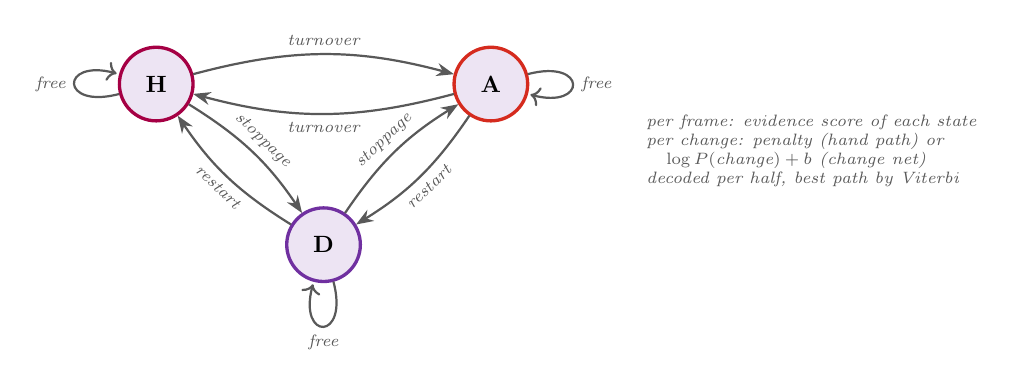
\begin{tikzpicture}[scale=0.85,transform shape,
                    state/.style={circle,draw=decline,fill=dec,very thick,minimum size=11mm,font=\bfseries}]
  \node[state,draw=barca] (H) at (0,0) {H};
  \node[state,draw=athletic] (A) at (5,0) {A};
  \node[state] (D) at (2.5,-2.4) {D};
  \draw[arr,bend left=15] (H) to node[note,above]{turnover} (A);
  \draw[arr,bend left=15] (A) to node[note,below]{turnover} (H);
  \draw[arr,bend left=12] (H) to node[note,above,sloped]{stoppage} (D);
  \draw[arr,bend left=12] (D) to node[note,below,sloped]{restart} (H);
  \draw[arr,bend left=12] (A) to node[note,below,sloped]{restart} (D);
  \draw[arr,bend left=12] (D) to node[note,above,sloped]{stoppage} (A);
  \draw[arr] (H) edge[loop left] node[note,left]{free} (H);
  \draw[arr] (A) edge[loop right] node[note,right]{free} (A);
  \draw[arr] (D) edge[loop below] node[note,below]{free} (D);
  \node[note,align=left,anchor=west] at (7.2,-1.0) {per frame: evidence score of each state\\
     per change: penalty (hand path) or\\ \quad $\log P(\text{change}) + b$ (change net)\\
     decoded per half, best path by Viterbi};
\end{tikzpicture}
\caption{The three-state decoder. Staying in a state is free; every change pays. This is what turns
noisy per-frame evidence into long, clean possessions.}
\label{fig:hmm}
\end{figure}

% ----------------------------------------------------------------
\section{The two sequence networks}\label{sec:nets}

The change network and the short-possession network share one architecture (Figure~\ref{fig:arch}).
Inputs are per-frame channels: 13 shared ball channels (position, height, velocity, speed,
acceleration, seen, gap, hand-path D, dead-head P, out, hold) and 17 per team (distances of the
three nearest players, counts within 2 / 5 / 10\,m, speed and direction toward the ball, centroid,
spread, touch P, first-stage and refiner P, the vote). c1dld adds two duel channels per team:
\code{ctl}, how closely the team's nearest player moves with the ball, and \code{keep}, how long the
same player has stayed within 3\,m. They are trained on 20-second random crops with home/away swap
augmentation, on the 84 external matches (SkillCorner 20 + PFF 64, plus DFL weighted $\times5$ for
c1dld), in four fixed folds plus one model on all matches; the deployed model is the
all-matches one.

\begin{figure}[!htbp]
\centering
\resizebox{0.92\linewidth}{!}{%
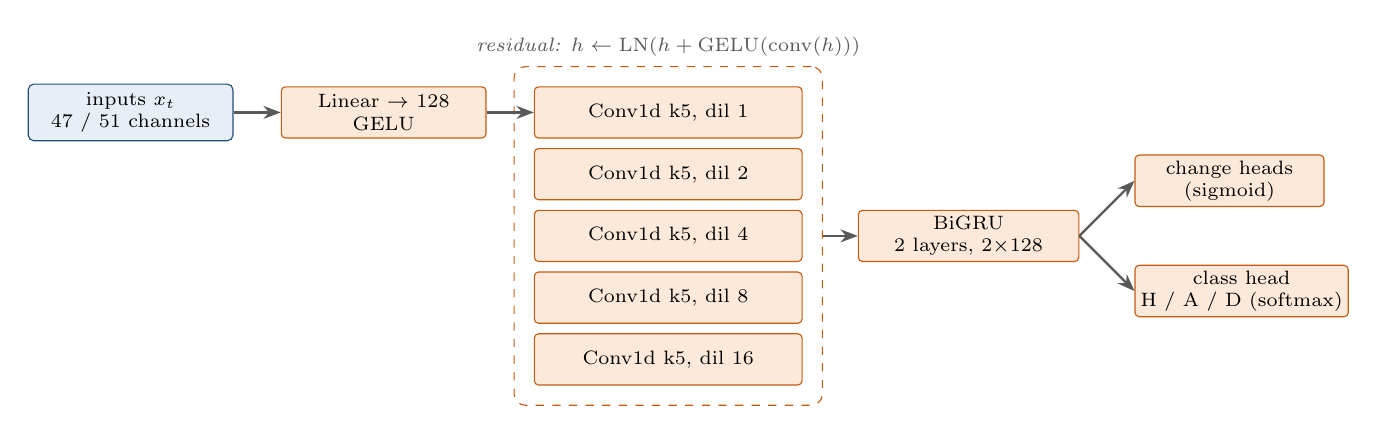
\begin{tikzpicture}[node distance=3mm]
  \node[box,minimum width=26mm,minimum height=6.5mm,font=\scriptsize] (x) {inputs $x_t$\\ 47 / 51 channels};
  \node[layer,right=6mm of x] (lin) {Linear $\to$ 128\\ GELU};
  \node[layer,right=6mm of lin,minimum width=34mm] (c1) {Conv1d k5, dil 1};
  \node[layer,below=1.2mm of c1,minimum width=34mm] (c2) {Conv1d k5, dil 2};
  \node[layer,below=1.2mm of c2,minimum width=34mm] (c3) {Conv1d k5, dil 4};
  \node[layer,below=1.2mm of c3,minimum width=34mm] (c4) {Conv1d k5, dil 8};
  \node[layer,below=1.2mm of c4,minimum width=34mm] (c5) {Conv1d k5, dil 16};
  \begin{scope}[on background layer]
    \node[draw=learnline,dashed,rounded corners,fit=(c1)(c5),inner sep=2.5mm,
          label={[note]above:residual: $h \leftarrow \mathrm{LN}(h + \mathrm{GELU}(\mathrm{conv}(h)))$}] (res) {};
  \end{scope}
  \node[layer,right=7mm of c3,minimum width=28mm] (gru) {BiGRU\\ 2 layers, 2$\times$128};
  \node[layer,right=7mm of gru,minimum width=24mm,yshift=7mm] (h1) {change heads\\ \scriptsize (sigmoid)};
  \node[layer,right=7mm of gru,minimum width=24mm,yshift=-7mm] (h2) {class head\\ \scriptsize H / A / D (softmax)};
  \draw[arr] (x) -- (lin);
  \draw[arr] (lin) -- (c1);
  \draw[arr] (res.east |- c3) -- (gru);
  \draw[arr] (gru.east) -- (h1.west);
  \draw[arr] (gru.east) -- (h2.west);
\end{tikzpicture}}

\vspace{3mm}
\small
\begin{tabularx}{\linewidth}{@{}l>{\raggedright\arraybackslash}X>{\raggedright\arraybackslash}X@{}}
\toprule
 & \textbf{Change network (c1dld)} & \textbf{Short-possession network (s1, s1b, s1nz)} \\
\midrule
Change heads & 5 Gaussian targets ($\sigma$ = 2 frames) at the first frame of a new state:
               turnover to H, to A, stoppage, restart to H, to A
             & 6 targets: inside / start / end of a possession shorter than 5\,s, per team \\
Class head   & H / A / D per frame & H / A / D per frame \\
Use          & mixed with the base, Viterbi with change transitions
             & ensemble mean $\to$ spells $\to$ XGBoost keep check $\to$ edges snapped \\
Members      & one model (all matches) & three variants; s1nz without ball height \\
\bottomrule
\end{tabularx}
\caption{Shared architecture: a per-frame projection, five residual dilated convolutions
(receptive field about $\pm$2.5\,s) for fine timing, and a two-layer bidirectional GRU over the whole
crop for context. The heads differ.}
\label{fig:arch}
\end{figure}

\textbf{Why a change network.} The question the challenge asks is \emph{when} possession changes
hands. Labelling frames and patching spells afterwards answers it indirectly; c1dld scores the
changes themselves. Held out, the first change net gained +0.017 to +0.022 \sF{} on every external
set over the short-net version, and the final c1dld +0.028 to +0.055 (Table~\ref{tab:external}).

\textbf{Why the check.} The short network alone fires on noise. Spells are generated loosely
(threshold 0.6) and an XGBoost classifier, trained on held-out spells with IoU $\geq$ 0.5 as the
label, decides which to keep. It lifted the share of caught short possessions on external data from
19\% to 44\%.

% ----------------------------------------------------------------
\section{Possession rules implemented}

\begin{itemize}
  \item \textbf{A possession} is a maximal run of one team with the ball alive. \code{H H D D H H} is
        two possessions; \code{H H A A} is two.
  \item \textbf{Control, not proximity.} The last team to touch the ball decides a change of team;
        team evidence decays with distance from the ball.
  \item \textbf{Loose balls and duels.} A touch without control (a deflection, a lost aerial duel)
        does not by itself change possession. Backdating applies only when the previous touch was
        weak, nothing happened in between and the ball was loose. The duel channels let the change
        network tell the player who runs with the ball from the one who only reached it.
  \item \textbf{Keeper holds.} A keeper holding the ball is never D during the hold (up to 8\,s), even
        through a tracking gap; the ball going untracked in the keeper's hands was an early error.
  \item \textbf{Restarts.} The tagged team of a set piece, or for an unflagged throw-in the side the
        ball left on, gives the restart's first possessor; passes among slow players during a
        stoppage are not a possession (restart handover).
  \item \textbf{Dead ball} is a stoppage, never a possession. Learned D can be added to live play;
        removing D is blocked wherever the ball was seen out of play.
  \item \textbf{Short possessions} (a long kick, then one contested touch) come only from spells the
        independent check accepts, so the decoder is not pushed into flicker.
\end{itemize}

% ----------------------------------------------------------------
\section{Keeper-swap correction}\label{sec:keeper}

The automatic tracker sometimes swaps a goalkeeper's identity with an outfield slot of the other
team: the keeper's track vanishes, reappears seconds later tens of metres away in the other goal,
while the real keeper of that goal freezes. \code{pipeline/track\_fix.fix\_teleports} finds this from
physics rather than position:

\begin{center}
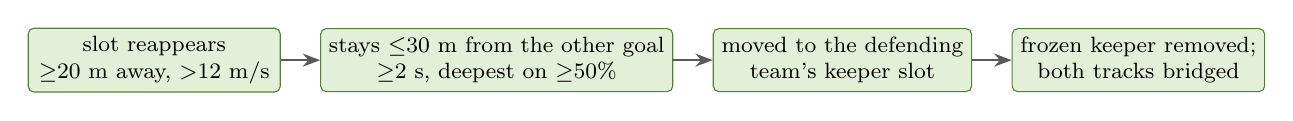
\begin{tikzpicture}[node distance=4mm and 5mm]
  \node[rbox,minimum width=32mm] (a) {slot reappears\\ $\geq$20 m away, $>$12 m/s};
  \node[rbox,minimum width=36mm,right=of a] (b) {stays $\leq$30 m from the other goal\\ $\geq$2 s, deepest on $\geq$50\%};
  \node[rbox,minimum width=32mm,right=of b] (c) {moved to the defending\\ team's keeper slot};
  \node[rbox,minimum width=32mm,right=of c] (d) {frozen keeper removed;\\ both tracks bridged};
  \draw[arr] (a) -- (b); \draw[arr] (b) -- (c); \draw[arr] (c) -- (d);
\end{tikzpicture}
\captionof{figure}{The teleport rule (variant \code{\_kt}). Over the full match: 16 teleports, 2 real
keeper swaps, 244\,s reassigned.}
\end{center}

It changes 27.6\,s of labels in total. On the public window it costs 0.038 \sF: before the fix,
the swapped tracking happened to create a short possession that matches a true one. We adopted it
anyway because it is correct tracking, and it is the base of every later version.

% ----------------------------------------------------------------
\section{Results}

\begin{figure}[!htbp]
\centering
\begin{minipage}[b]{0.6\linewidth}
\centering
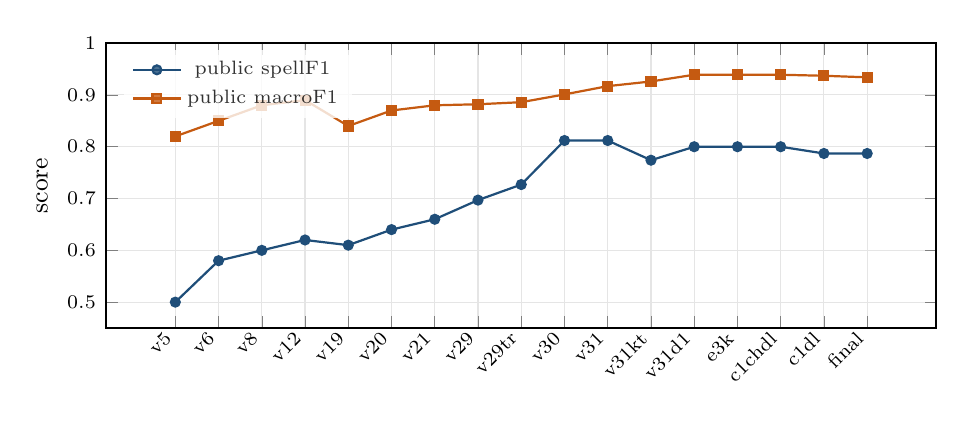
\begin{tikzpicture}
\begin{axis}[
  width=\linewidth, height=5.2cm,
  symbolic x coords={v5,v6,v8,v12,v19,v20,v21,v29,v29tr,v30,v31,v31kt,v31d1,e3k,c1chdl,c1dl,final},
  xtick=data, x tick label style={rotate=45,anchor=east,font=\scriptsize},
  ymin=0.45, ymax=1.0, ytick={0.5,0.6,0.7,0.8,0.9,1.0},
  ylabel={score}, ylabel style={font=\small}, tick label style={font=\scriptsize},
  grid=major, grid style={draw=gray!20},
  legend style={at={(0.02,0.98)},anchor=north west,font=\scriptsize,draw=none,fill=white,fill opacity=0.8},
  mark size=1.6pt, thick]
\addplot[color=accent,mark=*] coordinates {
  (v5,0.50) (v6,0.58) (v8,0.60) (v12,0.62) (v19,0.61) (v20,0.64) (v21,0.66) (v29,0.697)
  (v29tr,0.727) (v30,0.812) (v31,0.812) (v31kt,0.774) (v31d1,0.800) (e3k,0.800) (c1chdl,0.800)
  (c1dl,0.787) (final,0.787)};
\addlegendentry{public \sF}
\addplot[color=learnline,mark=square*] coordinates {
  (v5,0.82) (v6,0.85) (v8,0.88) (v12,0.89) (v19,0.84) (v20,0.87) (v21,0.88) (v29,0.882)
  (v29tr,0.886) (v30,0.901) (v31,0.917) (v31kt,0.926) (v31d1,0.939) (e3k,0.939) (c1chdl,0.939)
  (c1dl,0.937) (final,0.934)};
\addlegendentry{public \mF}
\end{axis}
\end{tikzpicture}
\end{minipage}\hfill
\begin{minipage}[b]{0.38\linewidth}
\centering
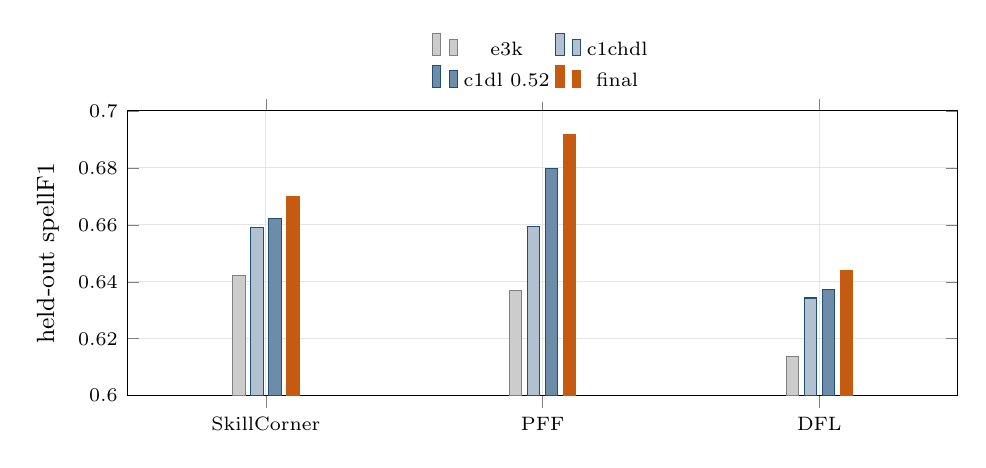
\begin{tikzpicture}
\begin{axis}[
  ybar, bar width=4.5pt, width=\linewidth, height=5.2cm,
  symbolic x coords={SkillCorner,PFF,DFL}, xtick=data, enlarge x limits=0.25,
  ymin=0.60, ymax=0.70, ytick={0.60,0.62,0.64,0.66,0.68,0.70},
  yticklabel style={/pgf/number format/fixed,/pgf/number format/precision=2},
  ylabel={held-out \sF}, ylabel style={font=\small},
  tick label style={font=\scriptsize}, grid=major, grid style={draw=gray!20},
  legend style={at={(0.5,1.03)},anchor=south,legend columns=2,font=\scriptsize,draw=none}]
\addplot[fill=gray!40,draw=gray] coordinates {(SkillCorner,0.6421) (PFF,0.6370) (DFL,0.6139)};
\addplot[fill=accent!35,draw=accent] coordinates {(SkillCorner,0.6589) (PFF,0.6594) (DFL,0.6343)};
\addplot[fill=accent!65,draw=accent] coordinates {(SkillCorner,0.6622) (PFF,0.6798) (DFL,0.6372)};
\addplot[fill=learnline,draw=learnline] coordinates {(SkillCorner,0.6699) (PFF,0.6916) (DFL,0.6438)};
\legend{e3k, c1chdl, c1dl 0.52, final}
\end{axis}
\end{tikzpicture}
\end{minipage}
\caption{\textbf{Left:} the public five-minute window over the version history. These 17 possessions
are a correctness check, not the selection criterion. \textbf{Right:} held-out \sF{} on the external
sets for the last four submissions (Table~\ref{tab:external}). From \code{v31\_d1} on, versions were
chosen on held-out data, where every step improves all three sets even when the public score is flat
or drops.}
\label{fig:history}
\end{figure}

\begin{table}[!htbp]
\centering\small
\begin{tabular}{@{}lcccc@{}}
\toprule
version & SkillCorner & PFF & DFL & public \sF{} / \mF \\
\midrule
\code{v31\_d1\_e3k\_kt} (short-net spells)          & 0.6421 & 0.6370 & 0.6139 & 0.800 / 0.939 \\
\code{v31\_d1\_c1chdlm\_e3k\_kt} (first change net) & 0.6589 & 0.6594 & 0.6343 & 0.800 / 0.939 \\
\code{v31\_d1\_c1dlm052\_e3k\_kt} (+ DFL $\times5$) & 0.6622 & 0.6798 & 0.6372 & 0.787 / 0.937 \\
\textbf{\code{v31\_d1\_c1dldm05\_e3k\_kt} (+ duel inputs)} & \textbf{0.6699} & \textbf{0.6916} & \textbf{0.6438} & 0.787 / 0.934 \\
\bottomrule
\end{tabular}
\caption{Held-out \sF{} on external matches (each match scored by models that never saw it) for
the last four submissions. The final version wins 82 matches and loses 7 against the one before it.}
\label{tab:external}
\end{table}

\textbf{Full match (aggregate):} 218 possessions of mean 15.3\,s, 39\% of team changes direct
(team to team, no stoppage between), 47.3\% D within the halves. The file has no \code{X}: frames
outside the halves, which are never graded, carry \code{D}.

% ----------------------------------------------------------------
\section{Assets: used and dropped}

\begin{table}[!htbp]
\centering\small
\begin{tabularx}{\linewidth}{@{}>{\raggedright\arraybackslash}p{3.6cm}>{\raggedright\arraybackslash}X>{\raggedright\arraybackslash}p{4.2cm}@{}}
\toprule
asset & use & outcome \\
\midrule
Automatic tracking (ATD) & the only positional input & \textbf{kept}, keeper swaps corrected \\
Smart Tagging & restart windows and teams, set-piece codes & \textbf{kept} at low weight \\
Homography / broadcast video & ball detection with pretrained YOLO models & \textbf{dropped}: noisier than the tracking ball (public 0.58--0.61 vs 0.77) \\
DFL open data (7 matches) & touch network, first stage, dead head, change net & \textbf{kept}: real tracking, provider possession flags, our gap pattern grafted in \\
SkillCorner open data (20) & short net, change net, dead head, validation & \textbf{kept} \\
PFF FC World Cup 2022 (64) & short net, change net, dead head, validation & \textbf{kept}: largest source of short possessions \\
Metrica sample games (3) & early validation & \textbf{dropped}: reconstructed ball, models trained on it transfer badly (public 0.49 / 0.67) \\
\bottomrule
\end{tabularx}
\caption{Data assets.}
\end{table}

\textbf{Methods tried and dropped} (each on held-out external matches): semi-Markov decoding with
explicit possession lengths (short possessions are limited by the evidence, not the decoder); MBR
decoding of the team stage (nested $-$0.003 on DFL); per-player set encoder as refiner input (+0.0063
vs +0.0085 for the simpler inputs); learned ball filling in tracking gaps as change-net input (no
gain over the original ball); loose-ball memory inputs (level on external data); protecting base
turnovers in the change-net mix (lost on external data); ball-free motion inputs for gap frames (no gain
over the dead head). \textbf{Cloud LLMs} were used as coding assistants only and saw aggregate scores
and counts, never match data.

% ----------------------------------------------------------------
\section{Limitations and next steps}

\begin{itemize}
  \item \textbf{Short possessions after a long ball} remain the weakest spot (a deep kick followed by
        one contested touch). Two of the public window's short possessions (0.8\,s and 1.3\,s) are
        missed by every version. Next: an air-ball flight and landing signal and post-contact ball
        direction as change-net inputs.
  \item \textbf{Ball gaps.} The ball is unseen on 43\% of frames. Live frames with the ball unseen are
        called D too often (33--51\% on every external set); this is where most of the remaining
        D errors sit.
  \item \textbf{Domain shift.} External sets differ in ball quality and pace. Held-out scores of 0.64--0.69
        are a more honest estimate of the full-match score than the public 0.787, which rests on
        17 possessions.
  \item \textbf{Boundary timing.} Team changes have no bias but a spread (IQR about 1.3\,s on
        external data), so no constant shift helps. On external data restarts come about 0.6\,s late
        and stops early, but the public window shows the opposite, so we applied no shift.
  \item \textbf{Keeper-swap fix} is a targeted rule for one tracker failure, not general re-identification.
  \item \textbf{One match.} Settings are validated on 91 external matches, but only one match of this
        tracking system exists to apply them to.
\end{itemize}

% ----------------------------------------------------------------
\section{Reproduction}\label{sec:repro}

Repository: branch \code{mirac}. Python 3.12 with the pinned versions in
\code{requirements-submission.txt}; a CUDA GPU for steps 2--4. Unpack the data bundle under
\code{data/} (never committed). All models the chain loads are committed in \code{models/}.

\begin{lstlisting}[language=bash]
pip install -r requirements-submission.txt --extra-index-url https://download.pytorch.org/whl/cu130
export MTAH_VARIANT=_kt        # PowerShell: $env:MTAH_VARIANT="_kt"
python tools/ours_chain.py --dead models/dead_ext_d1 --name v31_d1
python tools/short_net.py ours --ens "s1,s1b,s1nz:bz" --ens-tag e3 \
       --check k1:0.6:0.3 --over-d --hi 0.7 --name v31_d1_e3k_rb
python tools/cn_ours_bd.py --tag c1dld --duel --nofill
python tools/cn_sweep.py ours --tags c1dld --alphas 0.5
python evaluation/validate_submission.py evaluation/results/v31_d1_c1dldm05_e3k_kt.csv
\end{lstlisting}

The last file is the submission (md5 \code{ae577f788b03e0f0313f3613470c7dc3}), copied to
\code{Tiki-Taka.csv}. It was rebuilt from scratch on 2026-11-16 with the training caches hidden and came
out byte-identical. Retraining the models (not needed to rebuild the file) is documented in
\code{JOURNAL.md}, which records every version, its command and its scores. All diagnostics in the
repository print aggregates only.

\end{document}
